\documentclass[
    % -- opções da classe memoir --
    12pt,               % tamanho da fonte
    openright,          % capítulos começam em pág ímpar (insere página vazia caso preciso)
    %twoside,            % para impressão em verso e anverso. Oposto a oneside
    oneside,
    a4paper,            % tamanho do papel. 
    % -- opções da classe abntex2 --
    %chapter=TITLE,     % títulos de capítulos convertidos em letras maiúsculas
    %section=TITLE,     % títulos de seções convertidos em letras maiúsculas
    %subsection=TITLE,  % títulos de subseções convertidos em letras maiúsculas
    %subsubsection=TITLE,% títulos de subsubseções convertidos em letras maiúsculas
    % para pacote url reconhecer hifens como separador
    hyphens,
    paginasA3,  % indica que vai utilizar paginas em A3 
    GLOSSARIO, % gerar glossario a partir do arquivo defs-glossario.tex
    TODO, % indica que deve apresentar lista de pendencias 
    % -- opções do pacote babel --
    english,            % idioma adicional para hifenização
    brazil           % o último idioma é o principal do documento
    ]{ifsp-spo-inf-ctds} % ajustar de acordo com o modelo desejado para o curso

% ---
% Informações de dados para CAPA e FOLHA DE ROSTO
% ---
\titulo{STUDY FLOW}

% Trabalho em Equipe
% ver também https://github.com/abntex/abntex2/wiki/FAQ#como-adicionar-mais-de-um-autor-ao-meu-projeto
\renewcommand{\imprimirautor}{
\begin{tabular}{lr}
Kevin Klein & SP3096289 \\
Leonardo Tumani & SP309474X \\
Luiz Fernando & SP3096301\\
Ruan de Souza  & SP3069672 \\
Pedro Dias & SP3099211 \\
\end{tabular}
}


\disciplina{PI1A5 - Projeto Integrado I}

\preambulo{Desenho da aplicação para disciplina de PI1A5}

\data{2024}

% Definir o que for necessário e comentar o que não for necessário
% Utilizar o Nome Completo, abntex tem orientador e coorientador
% então vão ser utilizados na definição de professor
\renewcommand{\orientadorname}{Professor:}
\orientador{JOHNATA SOUZA SANTICIOLI}


% ---


% informações do PDF
\makeatletter
\hypersetup{
        %pagebackref=true,
        pdftitle={\@title}, 
        pdfauthor={\@author},
        pdfsubject={\imprimirpreambulo},
        pdfcreator={LaTeX with abnTeX2 using IFSP model},
        pdfkeywords={abnt}{latex}{abntex}{abntex2}{IFSP}{\ifspprefixo}{trabalho acadêmico}, 
        colorlinks=true,            % false: boxed links; true: colored links
        linkcolor=blue,             % color of internal links
        citecolor=blue,             % color of links to bibliography
        filecolor=magenta,              % color of file links
        urlcolor=blue,
        bookmarksdepth=4
}
\makeatother
% --- 

% carregando aqui referencias quando utilizando BIBLATEX
\IfPackageLoaded{biblatex}{%
\addbibresource{referencias.bib}
}{}

% ----
% Início do documento
% ----
\begin{document}



% Retira espaço extra obsoleto entre as frases.
\frenchspacing 

%somente para o exemplo, fica primeiro
% \todo[inline]{Remover texto informativo inicial}
% \newcommand{\urlmodelosimples}{https://www.sharelatex.com/project/58a3a66af9bb74023ba1bd56}

\newcommand{\urlmodelo}{\url{\urlmodelosimples}}

Esse documento foi feito a partir do modelo canônico do \abnTeX, o acesso ao PDF pode ser feito em 
\urlmodelo. A estrutura utilizada aqui foi um modelo utilizado no curso de Pós Graduação em Gestão de TI do \ac{ifsp}.
\todo{Remover texto informativo inicial}

%%A versão do sharelatex atualmente é a mais atualizada

%A versão atualizada da classe \ac{ifsp} para \LaTeX pode ser acessada em %\url{https://github.com/ivanfmartinez/latexlib/tree/master/ifsp}.

Este documento não pode ser considerado como um padrão a ser seguido em sua totalidade, ele tem como maior objetivo demonstrar como utilizar o \LaTeX para obter um documento atendendo ao máximo o padrão do \ac{ifsp} e \ac{abnt}.



\noindent\hrulefill



\newpage


% -- lista de pendencias gerada pelo todonotes
% -- altere opções do usepackage para remover na versão final....
% \listoftodos
% \todo[inline]{remover lista de todo da versão final...}
\newpage

% ----------------------------------------------------------
% ELEMENTOS PRÉ-TEXTUAIS
% ----------------------------------------------------------
\pretextual

% ---
% Capa
% ---
% \imprimircapa

\newcounter{todocounter}
\newcommand{\todonum}[2][]
{\stepcounter{todocounter}\todo[#1]{\thetodocounter: #2}}

\imprimirfolhaderosto

% ---
% inserir lista de ilustrações
% ---
%\pdfbookmark[0]{\listfigurename}{lof}
%\listoffigures*
%\cleardoublepage
% ---

% ---
% inserir lista de tabelas
% ---
%\pdfbookmark[0]{\listtablename}{lot}
%\listoftables*
%\cleardoublepage
% ---

% ---
% inserir lista de quadros
% ---
%\pdfbookmark[0]{\listofquadrosname}{loq}
%\listofquadros*
%\cleardoublepage
% ---

%% ---
% inserir lista de símbolos
% ---
\begin{simbolos}
  \item[$ \Gamma $] Letra grega Gama
  \item[$ \Lambda $] Lambda
  \item[$ \zeta $] Letra grega minúscula zeta
  \item[$ \in $] Pertence
\todo[inline]{ajustar utilizando glossaries}
\end{simbolos}
% ---

%\todo[inline]{Remover lista de simbolos se não for necessário}


% ---
% inserir o sumario
% ---
\pdfbookmark[0]{\contentsname}{toc}
\tableofcontents*
\cleardoublepage
% ---


% ----------------------------------------------------------
% ELEMENTOS TEXTUAIS
% ----------------------------------------------------------
\textual


\chapter{Introdução}

No Brasil, temos um importante instrumento de ascensão social através dos estudos, chamado “Concurso Público”. Muitas pessoas se dedicam para essa prova, pois através dela pode-se ter melhores ganhos e estabilidade financeira, além de depender do concurso um emprego sem demissão e plano de carreira atrativo. Com esse cenário, milhares de brasileiros tentam todos os anos a prova para esses concursos públicos para diferentes cargos e diversas esferas do poder público, mas com toda essa gama de provas e quantidade de concorrentes, como se preparar da melhor forma?}

Em nosso país, temos um mercado com grande potencial de crescimento e quando falamos de serviços para “concurseiros” (pessoas que prestam concursos públicos). Os serviços que tem a maior atratividade e público, são as plataformas de ensino direcionado para esse tipo de público. Com a Pandemia de \ac{covid} iniciada em 2020, essas plataformas tiveram uma mudança em seu modelo de negócio, precisando se adaptar ao modelo de \ac{ead}. 

Essa mudança no modelo de negócios das empresas do nicho de educação para concurso público, impactou os seus clientes, que agora consomem em maior quantidade serviços de educação online, aumentando ainda mais a possibilidade de novos serviços para esse tipo de cliente.

Com a migração de cursos antes no presencial, para agora online, os estudantes economizam tempo de deslocamento até a escola, tendo o serviço de aula na palma das mãos. E o tempo é justamente o ativo mais difícil para um estudante de concurso público, pois ele precisa conciliar suas atividades cotidianas e ainda seguir uma rotina de estudos e para iniciantes nesse mundo de concursos, além de tempo o que e como estudar se torna uma dificuldade maior ainda.

A tecnologia é uma grande aliada dos estudantes para ajudar a administrar esse cenário. Com o avanço de tecnologias de Inteligência Artificial, o que antes era um estudo e uma rotina sem parâmetros, pode ser otimizado e organizado de maneira muito mais fácil com a chegada desse recurso.


%Para criar uma sessão
\section{Objetivo}

Este projeto tem como objetivo ajudar os estudantes de concurso público a se organizarem com as matérias e rotina de estudos para um concurso público com o auxĺlio de tecnologias de Inteligência Artificial.

A plataforma em ambiente WEB permitirá que os estudantes enviem o edital em o qual irão prestar a prova e a partir desse edital a plataforma gere uma rotina de estudos personalizada pensando no maior ganho em sua jornada de estudos.

\end{itemize}

\section{Justificativa}

O projeto surge com o intuito de facilitação e otimização de tempo para os concurseiros. 
Com a utilização de recursos de inteligência artificial, métodos de estudo comprovados pela ciência e a criatividade, espera-se que a jornada e o resultado dos estudantes “concurseiros” seja mais fácil até o seu objetivo final que é a aprovação de um concurso.

A importância da aplicação vai além de sua praticidade, o seu valor agregado para o usuário é uma nova forma de utilizar a combinação entre estudo e tecnologia, que facilitará a  concretização da jornada da aprovação em um concurso público. 


\input{Std.1.2 - Análise de Concorrentes}



\input{Std.2 - Revisão da Literatura}
\chapter{GESTÃO DO PROJETO}

Nesta seção, serão apresentados os métodos escolhidos para a gestão do projeto e da equipe, com o objetivo de assegurar a melhor utilização possível do tempo, orçamento e recursos voltados para o projeto, para que esse possa ser concluído dentro do prazo estabelecido. Também serão levantados alguns riscos possíveis, afim de que com o conhecimento dessas possibilidades, medidas possam ser tomadas para evitá-los.  

\section{Formação da equipe}

A equipe foi formalizada durante as aulas da disciplina, porém já havia sido definida posteriormente. Todos os integrantes são alunos do curso de Tecnologia em Análise e Desenvolvimento de Sistemas, \acs{ifsp}, campus São Paulo. A equipe se baseia nos conhecimentos de cada um de seus membros com o objetivo de preencher as necessidades do projeto. Os participantes da equipe Noz são: 

\begin{itemize}
    \item \textbf{Kevin Klein}
    \item \textbf{Luiz Fernando Cavalcante de Faria}
    \item \textbf{Pedro Felipe da Silva Dias}
    \item \textbf{Ruan de Souza Cardoso Brito}
\end{itemize}

\subsection{Papéis}

Os papéis foram definidos através das habilidades dos membros , para que cada um pudesse atuar de maneira segura com seus conhecimentos, dessa maneira a organização e a fluidez do projeto são beneficiadas. As atividades são planejadas para que todos sejam responsáveis por alguma parte específica do projeto, podendo receber ajuda dos outros participantes caso seja necessário.

\subsection{Organização da atividades}

Dentro das atividades do projeto, a divisão está descrita no Quadro \ref{tab:Desenvolvimento }.
    \begin{quadro} [h]
    \centering
        \caption{Atividades de Desenvolvimento}\label{tab:Desenvolvimento }
 	\begin{tabular}{|c|c|c|c|c|}
        \hline
\textbf{Atividades}&\textbf{Kevin}&\textbf{Luiz}&\textbf{Pedro}&\textbf{Ruan} \\ \hline
Front-end &X & & &X \\ \hline
Back-end &X & &X & \\ \hline
Dados & &X & & \\ \hline
UX/UI & &X & & \\ \hline
Documentação & &X & &X \\ \hline
Inteligência Artificial &X & &X &\\ \hline
\end{tabular}
         \fonte{Os autores.}
    \end{quadro}


Além das atividades de desenvolvimento, as tarefas de gestão e planejamento foram divididas conforme o Quadro \ref{tab:Gestão }



    \begin{quadro} [h]
            \centering
 	    \caption{Atividades de gestão e planejamento} \label{tab:Gestão }



        \begin{tabular}{|c|c|c|c|c|}
    \hline
    \textbf{Atividades}&\textbf{Kevin}&\textbf{Luiz}&\textbf{Pedro}&\textbf{Ruan} \\    \hline
    SVN &X & & & \\ \hline
    LaTex & &X & & \\  \hline
    Blog & & & &X \\ \hline
    Youtube & & & &X \\ \hline
    Contato Orientador & & &X & \\ \hline
    Kanbam &X & & & \\ \hline
    Apresentações & &X & & \\ \hline
        \end{tabular}
            \fonte{Os autores.}
    \end{quadro}


\section{Gestão de tempo e desenvolvimento}

A equipe decidiu aderir à utilização do Scrum como \textit{framework} de gerenciamento, a fim de melhorar a organização durante o desenvolvimento do projeto. Ele foi escolhido pela sua eficiência e ampla utilização por diversas empresas no mercado, além de ser conhecido pelos integrantes do grupo, o que facilita sua implementação.  Além disso também optamos pela utilização do Kanban, para garantir a eficiência na realização das tarefas e o cumprimento dos prazos.

\subsection{Scrum}

O \textit{Scrum} é uma metodologia de desenvolvimento ágil amplamente empregada para lidar com a complexidade na criação de produtos. Este método valoriza a colaboração, a autonomia da equipe e a entrega progressiva e iterativa. Composto por uma série de práticas, papéis e artefatos, o Scrum promove a eficácia e a qualidade do trabalho realizado, impulsionando a entrega de valor de forma consistente ao longo do tempo.

\subsection{Kanban}

O Kanban é uma metodologia de gestão visual que teve origem no Japão e ganhou popularidade em diversos setores, como desenvolvimento de software, manufatura e serviços. O termo "Kanban" significa "sinal visual" em japonês, e essa abordagem se baseia na utilização de cartões ou post-its para representar unidades de trabalho e visualizar o fluxo do processo. Essa metodologia visa proporcionar transparência sobre o trabalho em andamento e controlar o \ac{wip} para otimizar a eficiência do sistema.

\section{Gestão de comunicação}
A comunicação é parte essencial para que tudo corra bem no projeto. Foram utilizados alguns meios para realizar esse diálogo entre a equipe.

O meios de comunicação utilizados internamente foram o  Whatsapp, aplicativo de mensagens instantâneas  e chamadas de voz, foi usado para troca de mensagens durantes as semanas, a fim de proporcionar agilidade e facilidade na comunicação, e o Discord, que é uma aplicação voltada para a comunicação, principalmente de grupos e comunidades, foi usado para as reuniões realizadas semanalmente.

Para a comunicação com o público foi criado um blog, na plataforma Blogger, onde são compartilhadas as atualizações semanais e informações relevantes sobre o projeto.

 \begin{figure}[!htb]
 	    \centering
 	    \caption{\label{logo}QR Code do Blog}
 	    
\includegraphics[width=5cm]{img/qrcode-blog.png}
 	    \fonte{Os autores.}
\end{figure}
\FloatBarrier

Além do blog, é possível acompanhar o desenvolvimento do projeto e das apresentações pelos vídeos presentes no canal do Youtube dedicado ao projeto.

 \begin{figure}[!htb]
 	    \centering
 	    \caption{\label{logo}QRCode do Youtube}
 	    
\includegraphics[width=5cm]{img/qrcode-youtube.png}
 	    \fonte{Os autores.}
\end{figure}
\FloatBarrier

\section{Análise de riscos}

Em todo projeto, riscos de todos os tipos e magnitudes podem ocorrer, impactando de forma significativa o andamento do projeto. 
Para a cosntrução do Studyflow, foram mapeados os riscos, o nível de impacto e a resposta aos mesmos, todos eles descritos no Quadro \ref{tab: Riscos}.

\begin{quadro} [h] % -- H posiciona exatamente no local em que foi inserido
    \centering
    \caption{Análise de Riscos}\label{tab: Riscos}
      
       \begin{tabular}{|c|c|c|}
       \hline
Risco &Nivel de Impacto &Resposta \\ \hline
Desistência pessoal &Alto &Aceitar \\ \hline
Problemas de Saúde &Alto &Aceitar \\ \hline
Conflitos Interpessoais &Médio &Mitigar \\ \hline
Comprometimento com outras tarefas &Médio &Mitigar \\ \hline
Mudança de Requisitos &Alto &Eliminar \\ \hline
Falhas de comunicação &Alto &Eliminar \\ \hline
Falta de conhecimento técnico &Médio &Mitigar \\ \hline
Problemas com conexão de rede &Baixo &Aceitar \\ \hline
Problemas com Hardware &Baixo &Aceitar \\ \hline
Escopo mal definido &Alto &Mitigar \\ \hline
Desempenho insastisfatório &Médio &Mitigar \\ \hline
Falhas de segurança &Médio &Mitigar \\ \hline
Falha em tecnologias externas &Médio &Aceitar \\ \hline
Problemas com o modelo de IA &Alto &Eliminar \\ \hline

\end{tabular}

\fonte{Os autores.}
\end{quadro}


Segue abaixo uma breve explicação sobre cada um dos possíveis riscos ao projeto:

\begin{itemize}
    \item \textbf{Desistência pessoal:} Membros da equipe abandonam o projeto, causando lacunas na expertise e sobrecarregando os membros restantes.
    \item \textbf{Problemas de saúde:} Membros da equipe enfrentam problemas de saúde que afetam sua capacidade de contribuir para o projeto.
    \item \textbf{Conflitos interpessoais:} Desentendimentos ou tensões entre membros da equipe prejudicam a colaboração e a eficiência do projeto.
    \item \textbf{Comprometimento com outras tarefas:} Membros da equipe têm prioridades divididas entre várias tarefas ou projetos, resultando em atrasos ou falta de dedicação ao projeto em questão.
    \item \textbf{Mudança de requisitos:} Alterações nos requisitos do projeto após o início do desenvolvimento, levando a retrabalho e atrasos.
    \item \textbf{Falhas na comunicação:} Comunicação inadequada entre membros da equipe, clientes ou partes interessadas, levando a mal-entendidos e erros.
    \item \textbf{Falta de conhecimento técnico:} Membros da equipe não possuem as habilidades ou conhecimentos necessários para concluir com sucesso determinadas tarefas ou aspectos do projeto.
    \item \textbf{Problemas com conexão de rede:} Problemas com a conexão de rede afetam a colaboração remota ou o acesso a recursos necessários para o projeto.
    \item \textbf{Falhas de hardware:} \textit{Hardware} essencial para o projeto falha, causando interrupções no desenvolvimento ou perda de dados.
    \item \textbf{Escopo mal definido:} Requisitos do projeto não estão claramente definidos desde o início, levando a confusão e revisões frequentes.
    \item \textbf{Desempenho insatisfatório:} O produto final não atende às expectativas de desempenho dos usuários, levando à insatisfação e possível rejeição.
    \item \textbf{Falha de segurança:} Vulnerabilidades de segurança no sistema comprometem a integridade ou a confidencialidade dos dados, resultando em riscos para os usuários e para a empresa.
    \item \textbf{Falha em tecnologias externas:} Dependência de tecnologias externas que podem falhar ou não atender às expectativas, afetando o desenvolvimento ou o funcionamento da aplicação.
    \item \textbf{Problema no treinamento da \acs{ia}:} Dificuldades no treinamento de sistemas de inteligência artificial para alcançar os resultados desejados, resultando em desempenho inadequado ou inexato.
\end{itemize}


\chapter{DESENVOLVIMENTO DO PROJETO}
\section{Arquitetura da solução}
O projeto web é dividido em duas camadas principais, sendo elas o front-end, responsável pela estilização da plataforma e interação com o usuário, e o back-end, responsável pela aplicação das regras de negócio, gestão das informações em um banco de dados, e pela lógica de execução em si da plataforma.

 \begin{figure}[!htb]
 	    \centering
 	    \caption{\label{logo}Arquitetura}
 	    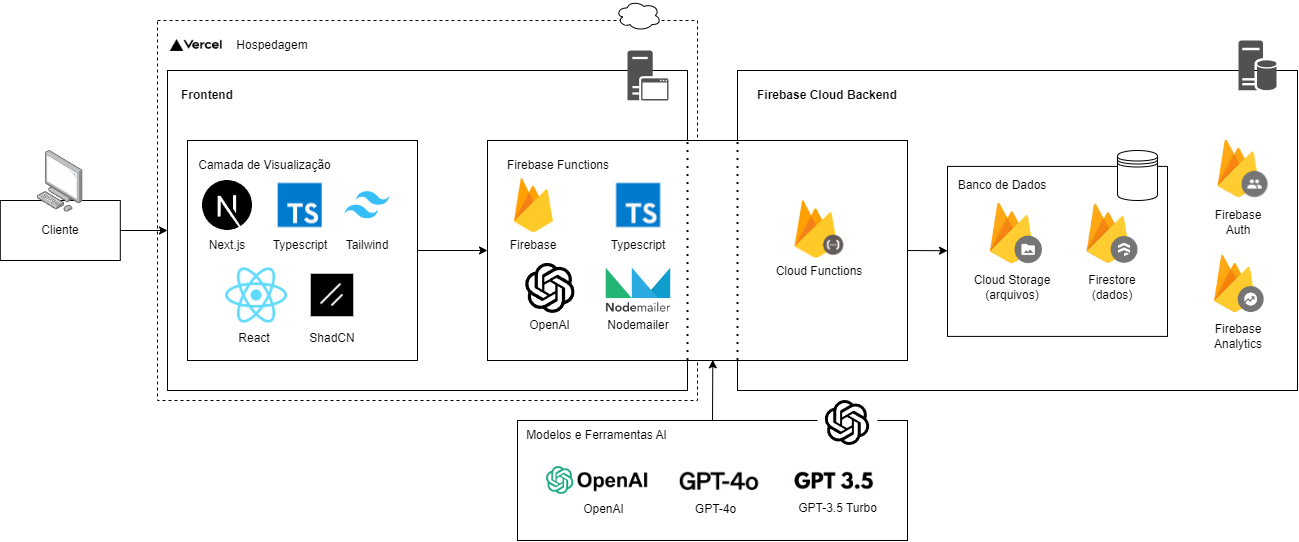
\includegraphics[width=15cm]{img/infra-model.png}
 	    \fonte{Os autores.}
\end{figure}

\subsection{Front-end}
O Front-end é a interface da aplicação, construída com Next.js, um framework React que oferece otimizações de desempenho e server-side rendering para uma experiência de usuário mais rápida e fluida. No desenvolvimento da interface, são empregadas as seguintes tecnologias:

\begin{itemize}
    \item \textbf{Tailwind CSS} \newline
Tailwind CSS é uma ferramenta utilizada para a estilização da aplicação. Ele adota uma abordagem de "utility-first", o que significa que as classes CSS são utilizadas diretamente no HTML para estilizar os elementos. Isso proporciona uma experiência de desenvolvimento mais rápida e consistente, além de facilitar a manutenção do código.

    \item \textbf{ShadCN} \newline
ShadCN é uma coleção de componentes prontos que podem ser importados e customizados dentro do código. Esses componentes são escritos em Typescript e Tailwind CSS. Ele não é considerado uma biblioteca, já que é uma extensão do Radix, outra biblioteca de estilização para Javascript.

    \item \textbf{Moment} \newline
Moment.js é uma biblioteca popular para manipulação de datas e horas em JavaScript. Ela oferece uma ampla gama de funcionalidades para formatação, análise e manipulação de datas, tornando mais fácil trabalhar com informações temporais na aplicação.

    \item \textbf{Nodemailer} \newline
Nodemailer é uma biblioteca utilizada para enviar e-mails através de Node.js. Ela oferece uma interface simples e flexível para o envio de e-mails, permitindo configurar facilmente o servidor de e-mail, criar templates personalizados e enviar mensagens de forma assíncrona.

    \item \textbf{Framer Motion} \newline
Framer Motion é uma biblioteca de animações para React que facilita a criação de animações fluidas e responsivas em componentes da interface. Ela oferece uma API declarativa e intuitiva para definir animações de entrada, saída e transição, além de suportar gestos e interações do usuário.

    \item \textbf{PDF Viewer} \newline
PDF Viewer é uma biblioteca Javascript projetada especificamente para a leitura de arquivos em formato PDF enviados pelos usuários, dentro do NodeJS. Com uma série de ferramentas avançadas, oferece uma experiência de visualização personalizada e intuitiva desses documentos.

    \item \textbf{Google Generative AI} \newline
A biblioteca Google AI JavaScript SDK permite que os desenvolvedores usem os modelos de IA generativos de última geração do Google (como o Gemini) para criar recursos e aplicativos com tecnologia de IA.

    \item \textbf{Bibliotecas do Firebase} \newline
Dentro do Front-end, são utilizadas diversas bibliotecas do Firebase para interação com o Back-end e execução de funcionalidades como autenticação, armazenamento de dados e comunicação em tempo real. Algumas das bibliotecas comumente utilizadas incluem:
\begin{itemize}
    \item \textbf{firebase}
    \item \textbf{firebase-admin}
    \item \textbf{firebase-functions}
    \item \textbf{firebase-tools}
\end{itemize}

Essas bibliotecas fornecem uma integração simplificada entre o Front-end e o Back-end, permitindo o desenvolvimento de uma aplicação robusta e interativa.

\end{itemize}

\subsection{Back-end}
Para o Back-end, é utilizado Firebase, que fornece serviços de banco de dados, armazenamento, autenticação e hospedagem, entre outros, de forma simplificada. O Firebase permite uma configuração rápida e fácil, facilitando o desenvolvimento e a viabilização do projeto.
Dentro da plataforma do Firebase, são utilizadas as seguintes funcionalidades:

\begin{itemize}
\item \textbf{Firebase Auth} \newline
Para autenticação de usuários, permitindo login com e-mail, redes sociais, entre outros métodos.
\item \textbf{Firebase Firestore} \newline
Para armazenamento e gerenciamento de dados em tempo real, oferecendo um banco de dados NoSQL escalável e altamente disponível.
\item \textbf{Firebase Storage} \newline
Para armazenamento de arquivos, como imagens e vídeos, diretamente na infraestrutura do Firebase.
\end{itemize}

\subsection{Banco de dados}
O banco de dados da aplicação está contido nos serviços oferecidos pelo Firebase Realtime Database e Firestore, que são bancos de dados NoSQL escaláveis e altamente disponíveis. A comunicação entre as camadas, API externas e com o cliente são realizadas através do Protocolo HTTP e chamadas REST.
O banco de dados é estruturado da seguinte maneira, a fim de suportar a gestão das informações dentro da plataforma:

\begin{itemize}
    \item \textbf{Tabela users}
    
    \begin{itemize}
    \item \textbf{fullname:} Armazena o nome completo do usuário.
    \item \textbf{email:} Guarda o endereço de e-mail do usuário.
    \item \textbf{document:} Pode armazenar o documento de identificação do usuário, como CPF. 
    \item \textbf{noticeid:} Chave estrangeira que faz referência ao edital (notice) associado ao usuário.
    \end{itemize}
    
    \item \textbf{Tabela tasks}
    
    \begin{itemize}
    \item \textbf{title:} Título da tarefa.
    \item \textbf{description:} Descrição detalhada da tarefa.
    \item \textbf{contentid:} Chave estrangeira que referencia o conteúdo (content) associado à tarefa. 
    \item \textbf{difficultyid:} Chave estrangeira que referencia o nível de dificuldade da tarefa. 
    \item \textbf{hasfinished:} Indica se a tarefa foi concluída ou não.
    \item \textbf{userid:} Chave estrangeira que faz referência ao usuário que criou a tarefa. 
    \item \textbf{dayofweek:} Dia da semana em que a tarefa deve ser realizada.
    \item \textbf{startat:} Horário de início da tarefa.
    \item \textbf{finishat:} Horário de término da tarefa.
    \end{itemize}
    
    \item \textbf{Tabela difficulties}
    
    \begin{itemize}
    \item \textbf{name:} Nome do nível de dificuldade.
    \item \textbf{displayname:} Nome de exibição do nível de dificuldade.
    \end{itemize}
    
    \item \textbf{Tabela subjects (matérias)}
    \begin{itemize}
    \item \textbf{name:} Nome da matéria.
    \item \textbf{noticeid:} Chave estrangeira que faz referência ao edital (notice) associado à matéria.
    \end{itemize}
    
    \item \textbf{Tabela contents}
    \begin{itemize}
    \item \textbf{subjectid:} Chave estrangeira que referencia a matéria (subject) associada ao conteúdo. 
    \item \textbf{text:} Texto do conteúdo, que pode conter informações relevantes para estudo.
    \end{itemize}
    
    \item \textbf{Tabela notices (editais)}
    \begin{itemize}
    \item \textbf{name:} Nome do cargo ou edital.
    \item \textbf{filesrc:} Caminho para o arquivo do edital. 
    \item \textbf{userid:} Usuário que fez o upload do edita.
    \end{itemize}
    
\end{itemize}

Este modelo de banco de dados é projetado para permitir a associação de usuários a tarefas específicas, associadas a conteúdos de estudo e matérias específicas relacionadas aos editais. A inclusão de um nível de dificuldade (na tabela difficulties) proporciona uma maneira de classificar a complexidade das tarefas, enquanto a tabela notices permite o armazenamento e acesso aos editais relacionados aos estudos.

 \begin{figure}[!htb]
 	    \centering
 	    \caption{\label{logo}Modelo de classes do banco de dados}
 	    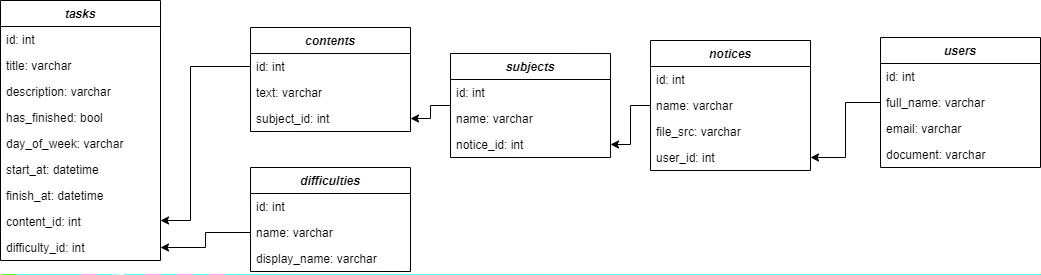
\includegraphics[width=15cm]{img/db-model.png}
 	    \fonte{Os autores.}
\end{figure}
\FloatBarrier

\subsection{Integrações}
Para a interpretação dos conteúdos pragmáticos dentro dos editais, faremos uso e customização dos modelos de inteligência artificial fornecidos pelo Google Gemini. O Gemini, anteriormente conhecido como Bard, é um chatbot desenvolvido pelo Google, baseado na família de modelos de linguagem LaMDA.
No contexto específico de nossa plataforma, contamos com dois modelos treinados para desempenhar funções cruciais:

\begin{itemize}
\item \textbf{Interpretação de Conteúdo de Edital e Geração de Matérias} \newline
Este modelo é encarregado de interpretar o conteúdo pragmático após a filtragem do edital fornecido pelo usuário. Ele irá identificar e extrair as matérias que serão cobradas no concurso, populando assim o banco de dados.

\item \textbf{Interpretação de Matérias e Geração de Tarefas e Rotinas de Estudo} \newline
 Com o banco de dados já contendo as matérias identificadas, este modelo entra em ação para gerar tarefas e rotinas de estudo personalizadas. Recebendo como entrada as matérias e conteúdos que o usuário ainda precisa estudar, ele irá gerar um cronograma de estudo detalhado, distribuindo as tarefas ao longo da semana de acordo com as necessidades e preferências do usuário.
\end{itemize}

Essas integrações permitem uma abordagem mais eficiente e personalizada no processo de estudo para concursos, aproveitando o poder dos modelos de linguagem avançados fornecidos pelo Google Gemini.

\subsection{Versionamento de Código}
O versionamento de código é uma prática fundamental no desenvolvimento de software, permitindo o controle e gerenciamento das alterações feitas ao longo do tempo em um projeto. Para isso, utilizaremos o GitHub como plataforma de versionamento, que oferece uma série de recursos poderosos para colaboração e controle de versões. No nosso ambiente de desenvolvimento, teremos um repositório principal hospedado no GitHub:

\textbf{Repositório do Front-end e Functions do Firebase:} \newline
Este repositório conterá o código-fonte do Front-end desenvolvido com Next.js, bem como as functions do Firebase utilizadas no Back-end. Será organizado de forma a separar claramente os diretórios relacionados ao Front-end e às functions do Firebase, mantendo uma estrutura de pastas intuitiva e coesa.

\textbf{Estratégia de Versionamento: Gitflow} \newline
Para gerenciar as diferentes etapas de desenvolvimento e garantir uma colaboração eficiente entre os membros da equipe, adotaremos a estratégia de versionamento Gitflow. Essa abordagem define um modelo de fluxo de trabalho baseado em branches, que facilita a organização das funcionalidades em desenvolvimento, testes e produção.
Principais Branches:

\begin{itemize}
\item \textbf{Main (ou Master):} Esta branch representa a versão estável e de produção do código. Todo o código que está pronto para ser implantado em ambiente de produção é mesclado nesta branch.

\item \textbf{Develop:} Esta branch é onde o desenvolvimento ativo ocorre. É a branch de integração para novas funcionalidades e correções de bugs. Todo o desenvolvimento é feito a partir desta branch.

\item \textbf{Feature Branches:} Para cada nova funcionalidade ou tarefa, uma nova branch de feature é criada a partir da branch develop. Esta branch é utilizada para implementar a funcionalidade de forma isolada, antes de ser integrada de volta à branch develop.
\end{itemize}
 
Adotando essa estratégia de versionamento com o Gitflow, garantimos um desenvolvimento organizado, facilitando a colaboração entre os membros da equipe e mantendo um histórico claro e estruturado das alterações feitas no código-fonte ao longo do tempo.

\subsection{Infraestrutura}
Para hospedagem, optaremos por utilizar os serviços especializados de hospedagem da Vercel para o Front-end e do Firebase para o Back-end customizado.

\textbf{Hospedagem do Front-end} \newline
A Vercel oferece um serviço de hospedagem altamente escalável e otimizado para aplicações Front-end, como o nosso desenvolvido com Next.js. Utilizando a plataforma da Vercel, podemos implantar e hospedar facilmente nosso Front-end, garantindo uma experiência de usuário rápida e confiável.

\textbf{Hospedagem do Back-end no Firebase} \newline
O Firebase oferece por padrão a hospedagem de seus serviços diretamente em sua plataforma, eliminando a necessidade de recorrer a soluções terceirizadas para essa finalidade. Essa integração nativa proporciona uma infraestrutura completa e integrada, capaz de suportar todas as necessidades de nossa aplicação de forma eficiente e escalável.

\subsection{Escalabilidade}
Tanto a Vercel quanto o Firebase oferecem opções de escalabilidade conforme as necessidades do projeto. No caso da Vercel, podemos facilmente escalar nossa aplicação Front-end de acordo com o aumento da demanda de tráfego. Já o Firebase, além de oferecer hospedagem escalável, também permite dimensionar automaticamente o banco de dados e outros serviços conforme necessário.

\subsection{Convenções e Padronização de Código}

Convenções são acordos ou regras estabelecidas para padronizar a forma como realizamos determinadas atividades ou interações. No contexto do desenvolvimento de software, as convenções de codificação são diretrizes estabelecidas para padronizar a escrita e a organização do código-fonte de uma aplicação. Elas definem como devemos nomear variáveis, formatar o código, documentar funcionalidades e adotar certas práticas de desenvolvimento.

Para esse projeto, iremos seguir com as seguintes convenções e padrões de código:

\begin{itemize}
    \item Nomenclatura de Variáveis e Funções:

Utilize nomes descritivos e significativos para variáveis e funções.
Prefira camelCase para nomes de variáveis e funções em JavaScript/TypeScript.

    \item Comentários:
Inclua comentários claros e concisos para explicar trechos de código complexos ou de difícil compreensão.
Evite comentários óbvios que apenas repetem o que o código faz.

    \item Indentação e Formatação:

Utilize uma tabulação consistente para indentação, preferencialmente com 2 ou 4 espaços.
Mantenha linhas de código com até 80-100 caracteres para facilitar a leitura em telas menores.
Organize o código de forma clara e coesa, utilizando espaços em branco para separar blocos lógicos.

    \item Tratamento de Erros:

Sempre inclua tratamento de erros adequado em pontos críticos do código.
Utilize try-catch para capturar e lidar com exceções de forma apropriada.

    \item Gerenciamento de Dependências:

Mantenha uma lista atualizada de todas as dependências e suas versões no arquivo de manifesto (como package.json).
Utilize um gerenciador de dependências confiável, como npm ou yarn, e evite adicionar dependências desnecessárias.

    \item Revisões de Código:

Realize revisões de código regulares entre os membros da equipe para identificar e corrigir problemas de qualidade, estilo e desempenho.
Mantenha um ambiente colaborativo e aberto para sugestões e melhorias no código.

\end{itemize}

\newpage

\subsection{Viabilidade Financeira e Planos de Upgrade}

Inicialmente, para a fase de desenvolvimento e testes, vamos utilizar os planos gratuitos oferecidos pela Vercel para hospedar nosso Front-end. Essa escolha nos permitirá iniciar o projeto de maneira ágil e econômica, facilitando a implantação e os testes iniciais da aplicação.

No entanto, para a fase de produção e lançamento oficial da plataforma, planejamos migrar para soluções pagas. Na Vercel, iremos adotar, inicialmente, o plano Pro, que oferece recursos adicionais, como escalabilidade aprimorada, limites maiores de "bandwidth" e de cachê de dados, além de suporte especializado. Isso garantirá um desempenho consistente e confiável da nossa aplicação em ambiente de produção, além de proporcionar um nível mais alto de serviço e suporte.

Já no Firebase, desde a fase de desenvolvimento iremos optar pelo plano pago Blaze. Isso se dá pois esse plano nos da acesso a serviços específicos da plataforma, como as Functions, funcionalidade que será essencial para o funcionamento da plataforma. Apesar de ser um plano pago, nossos custos iniciais serão baixos, pois o plano segue o formato "pay-as-you-go", ou seja, o faturamento da conta será conforme o uso da plataforma. A flexibilidade desse modelo de pagamento nos permitirá começar com custos mínimos e aumentar conforme o crescimento e a demanda da aplicação.

Os custos do Gemini AI ainda estão sendo levantados. Por se tratar de uma plataforma recente, o Gemini conta apenas com um plano gratuito, que possui limites de uso que se encaixam com o nosso uso durante o desenvolvimento, mas não para o cenário de produção. Apesar disso, o Gemini pretende lançar um plano pay-as-you-go, assim como o Firebase, que possui limites mais adequados para o lançamento da plataforma, mas que conta com um preço de entrada. 

Essas abordagens nos possibilitam começar com investimentos mínimos durante a fase de desenvolvimento, ajustando nossos gastos de acordo com o crescimento e a maturidade do projeto. Dessa forma, garantimos uma transição suave para o ambiente de produção, maximizando o valor entregue aos usuários finais e garantindo o sucesso contínuo da nossa aplicação.

\subsection{Planos de Assinatura e Expectativa Financeira}

Após a análise dos custos envolvidos na operação da plataforma, reconhecemos a necessidade de implementar um modelo de assinatura para garantir o acesso completo às ferramentas oferecidas pela nossa aplicação. Este modelo de assinatura será oferecido em formatos mensal e anual, proporcionando flexibilidade aos usuários de acordo com suas preferências e necessidades. Abaixo, detalhamos os planos disponíveis:

\textbf{Plano Gratuito}

Com o plano gratuito, o usuário terá acesso a todas as funcionalidades da plataforma. Porém, ele está limitado a fazer o upload de apenas um edital, e de utilizar a geração de tarefas por até 3 semanas. Dessa forma, o usuário pode ter uma experiência dentro da plataforma, e decidir se faz sentido ou não começar a pagar pelos serviços completos.

\textbf{Plano Pago}

Nosso Plano Pago oferece aos usuários acesso ilimitado a todas as funcionalidades e recursos avançados da plataforma. Com este plano, os usuários podem fazer o upload de múltiplos editais e aproveitar a geração ilimitada de tarefas.

Para cobrir os custos operacionais e garantir a sustentabilidade da plataforma, estimamos o preço mensal da assinatura em R\$24,99 e o preço anual em R\$249,90. Essa estrutura de preços proporciona aos usuários flexibilidade e economia, incentivando-os a aderir ao plano anual para obter um desconto significativo.
\input{Std.4.2 - Historias do usuário}
\section{Fases de Entrega}

As fases de entrega de um projeto são etapas fundamentais que conduzem o desenvolvimento de uma solução desde sua concepção até sua implementação e lançamento. Cada fase representa um marco importante no ciclo de vida do projeto, onde objetivos específicos são alcançados e progresso significativo é realizado.

Nossas fases de entrega planejadas são:

\begin{itemize}
\item Planejamento e Análise:
Nesta fase, são identificados os requisitos do projeto, definidos os objetivos e escopo, e elaborado o plano de projeto detalhado. Também é realizada uma análise de viabilidade técnica e financeira.

\item Prova de Conceito (PoC):

A \ac{poc} é uma fase inicial do projeto na qual são desenvolvidos protótipos ou demonstrações que validam a viabilidade técnica das principais funcionalidades da plataforma. Nesta fase, focamos em implementar um conjunto mínimo de recursos para validar a solução proposta e demonstrar sua viabilidade.

\item Desenvolvimento Iterativo:
Após o sucesso da \acs{poc}, o desenvolvimento da plataforma começa em etapas iterativas. Funcionalidades adicionais são implementadas em ciclos de desenvolvimento curtos, permitindo feedback contínuo e ajustes conforme necessário.

\item Testes e Qualidade:
Durante todo o processo de desenvolvimento, são realizados testes rigorosos para garantir que a plataforma atenda aos requisitos de qualidade e segurança. Isso inclui testes de unidade, integração, aceitação do usuário e segurança.

\item Implantação e Lançamento:
Após a conclusão do desenvolvimento e dos testes, a plataforma é implantada em um ambiente de produção e está pronta para ser lançada. Isso pode incluir a configuração de servidores, migração de dados e treinamento de usuários.

\item Monitoramento e Manutenção:
Após o lançamento, a plataforma é continuamente monitorada para garantir que esteja funcionando conforme o esperado. Também são feitas atualizações regulares e manutenção para corrigir bugs, adicionar novos recursos e melhorar a experiência do usuário.

\end{itemize}

\textbf{Prova de Conceito (PoC) Inicial:}
Na \acs{poc} inicial, nosso foco seria desenvolver um protótipo funcional da plataforma que demonstre as principais funcionalidades propostas. Isso pode incluir a autenticação de usuários, a criação de tarefas e a integração com serviços de terceiros, como o Firebase para o back-end e a Vercel para o front-end. A \acs{poc} permite validar a viabilidade técnica da solução proposta e identificar possíveis desafios ou obstáculos que precisam ser superados antes da implementação completa.

\textbf{Entrega Final da Plataforma:}

Na entrega final da plataforma, todos os recursos e funcionalidades planejados são implementados e testados completamente. Isso inclui a implementação completa e treinamento dos modelos de \acs{ia}, adequação a políticas de segurança, a integração com serviços de terceiros, como autenticação, armazenamento de dados e hospedagem, e a garantia de que a plataforma atenda aos requisitos de desempenho, escalabilidade e usabilidade. A entrega final marca o lançamento oficial da plataforma e seu uso pelos usuários finais.
\input{Std.4.4 - Segurança}


\begin{comment}

\chapter{Migrar do site}
% https://www.overleaf.com/learn/latex/Articles/How_to_write_in_Markdown_on_Overleaf
\todo[inline]{Coloquei como outro arquivo  pds.md para ficar mais facil de ajustar e remover o que precisar conforme formos ajustando}
\markdownInput{pds.md}

\end{comment}


% ----------------------------------------------------------
% Finaliza a parte no bookmark do PDF
% para que se inicie o bookmark na raiz
% e adiciona espaço de parte no Sumário
% ----------------------------------------------------------
\phantompart

% ----------------------------------------------------------
% ELEMENTOS PÓS-TEXTUAIS
% ----------------------------------------------------------
\postextual
% ----------------------------------------------------------

% ----------------------------------------------------------
% Referências bibliográficas
% ----------------------------------------------------------

\bibliography{referencias}

% ----------------------------------------------------------
% Glossário
% ----------------------------------------------------------
%
%
\ifdef{\printnoidxglossary}{
    \addcontentsline{toc}{chapter}{GLOSSÁRIO}
    \printnoidxglossary[style=glossario]
    %\printglossaries
}{}

%% ----------------------------------------------------------
% Apêndices
% Documentos gerados pelo próprio autor
% ----------------------------------------------------------

% ---
% Inicia os apêndices
% ---
\begin{apendicesenv}

% Imprime uma página indicando o início dos apêndices
\partapendices

% ----------------------------------------------------------
\chapter{Quisque libero justo}
% ----------------------------------------------------------

\lipsum[1-2]

% ----------------------------------------------------------
\chapter{Nullam elementum urna vel imperdiet sodales elit ipsum pharetra ligula
ac pretium ante justo a nulla curabitur tristique arcu eu metus}
% ----------------------------------------------------------
\lipsum[3-5]

\end{apendicesenv}
% ---

%% ----------------------------------------------------------
% Anexos
% Documentos gerados por outros autores
% ----------------------------------------------------------

% ---
% Inicia os anexos
% ---
\begin{anexosenv}

% Imprime uma página indicando o início dos anexos
\partanexos

% ---
\chapter{Manual todonotes}
\label{manual-todonotes}
% ---
\index{pdf}
% arquivo completo
\includepdf[pages=-,frame=true]{anexos/todonotes.pdf}

% ---
\chapter{Manual pdfpages(parcial)}
% ---
\index{pdf}
% somente algumas páginas
\includepdf[pages=1-3,frame=false]{anexos/pdfpages.pdf}

% ---
\chapter{Manual acronym(parcial)}
% ---
\index{pdf}
% somente algumas páginas
\includepdf[pages=1-3,frame=false]{anexos/acronym.pdf}


% ---
\chapter{Cras non urna sed feugiat cum sociis natoque penatibus}
% ---

\lipsum[1]



\end{anexosenv}



%---------------------------------------------------------------------

\end{document}